%\documentclass[a4paper,11pt,twoside,openright]{report}
\documentclass[a4paper,11pt,twoside]{report}


%%%%%%%%%%%%%%%%%%%%%%%%%%%%
% LINE SPACING:
\newcommand{\linespacing}{1.5}
\renewcommand{\baselinestretch}{\linespacing}
%%%%%%%%%%%%%%%%%%%%%%%%%%%%


%%%%%%%%%%%%%%%%%%%%%%%%%%%%
% BIBLIOGRAPHY STYLE:
\usepackage{cite}
\bibliographystyle{ieeetr}
%%%%%%%%%%%%%%%%%%%%%%%%%%%%


%%%%%%%%%%%%%%%%%%%%%%%%%%%%
% OTHER FORMATTING/LAYOUT DECLARATIONS:
\usepackage{amsmath}
\usepackage{amssymb}
\usepackage{comment}
\usepackage{physics}
% Graphics
\usepackage{feynmp-auto}
\usepackage{graphicx,color}
\usepackage{epstopdf}
\usepackage[british]{babel}
\usepackage[a4paper,top=2.5cm,bottom=2.5cm,left=4cm,right=2cm,headsep=10pt]{geometry}
\flushbottom
\usepackage{fancyhdr}
\fancypagestyle{plain}{
	\fancyhf{}
	\fancyhead[LE,RO]{\bfseries \thepage}
}
\pagestyle{plain}
\fancyhf{}
\renewcommand{\chaptermark}[1]{\markboth{#1}{}}
\fancyhead[LO,RE]{\bfseries \leftmark}
\fancyhead[LE,RO]{\bfseries \thepage}
\pagestyle{fancy}
\usepackage{array}
\usepackage{mhchem}
\usepackage{multirow}
\usepackage{ragged2e}
\usepackage{rotating}
\newcolumntype{A}{>{\centering\arraybackslash} m{0.125\textwidth}}
\newcolumntype{B}{>{\centering\arraybackslash} m{0.2\textwidth}}
\usepackage{caption}
\usepackage{subcaption}
%%%%%%%%%%%%%%%%%%%%%%%%%%%%


%%%%%%%%%%%%%%%%%%%%%%%%%%%%
% INPUT PATHS:
\makeatletter
\def\input@path{{/Users/booth/Desktop/LaTeXThesisTemplate/}}
\def\Ginput@path{{/Users/booth/Desktop/LaTeXThesisTemplate/}}
\makeatother
%%%%%%%%%%%%%%%%%%%%%%%%%%%%



%%%%%%%%%%%%%%%%%%%%%%%%%%%%
% HYPERREF
\usepackage[colorlinks,pdfusetitle,urlcolor=black,citecolor=black,linkcolor=black,bookmarksnumbered,plainpages=false]{hyperref}
% FOR PRINT VERSION, USE INSTEAD:
%\usepackage[pdfusetitle,bookmarksnumbered,plainpages=false]{hyperref}
%\usepackage{backref}
%\renewcommand{\backrefpagesname}{Cited on}
%%%%%%%%%%%%%%%%%%%%%%%%%%%%


%%%%%%%%%%%%%%%%%%%%%%%%%%%%
% CUSTOM COMMANDS:
\newcommand{\numu}{$\nu_\mu\ $}
%%%%%%%%%%%%%%%%%%%%%%%%%%%%


%%%%%%%%%%%%%%%%%%%%%%%%%%%%
% ACRONYMS:
\usepackage[acronym,nomain,nonumberlist]{glossaries}
\makeglossaries
\newacronym{ADC}{ADC}{Analogue to Digital Converter}
%%%%%%%%%%%%%%%%%%%%%%%%%%%%


%%%%%%%%%%%%%%%%%%%%%%%%%%%%
% BEGIN DOCUMENT
\begin{document}
%%%%%%%%%%%%%%%%%%%%%%%%%%%%


%%%%%%%%%%%%%%%%%%%%%%%%%%%%
% PREAMBLE: roman page num. i, ii, iii, ...
\pagenumbering{roman}
%%%%%%%%%%%%%%%%%%%%%%%%%%%%


%%%%%%%%%%%%%%%%%%%%%%%%%%%%
% TITLE PAGE:
\thispagestyle{empty}
\begin{flushright}

\includegraphics[width=6cm]{BaseDir/Plots/uslogo.pdf}
\end{flushright}	
\vskip40mm
\begin{center}
% TITLE
\huge\textbf{Thesis Title}
\vskip5mm
% AUTHOR
\Large\textbf{Firstname Surname}
\normalsize
\end{center}
\vfill
\begin{flushleft}
\large
% QUALIFICATION:
Submitted for the degree of Doctor of Philosophy \\
University of Sussex	\\
% DATE OF SUBMISSION:
Month YYYY
\end{flushleft}		
%%%%%%%%%%%%%%%%%%%%%%%%%%%%


%%%%%%%%%%%%%%%%%%%%%%%%%%%%
% DECLARATIONS:
\chapter*{Declaration}
I hereby declare that this thesis has not been and will not be, submitted in whole or in part to another University for the award of any other degree.
\vskip5mm
Signature:
\vskip15mm
% AUTHOR
Firstname Surname
%%%%%%%%%%%%%%%%%%%%%%%%%%%%


%%%%%%%%%%%%%%%%%%%%%%%%%%%%
% SUMMARY PAGE:
\thispagestyle{empty}
\newpage
\null\vskip10mm
\begin{center}
\large
\underline{UNIVERSITY OF SUSSEX}
\vskip20mm
% AUTHOR, QUALIFICATION:
%\textsc{Firstname Surname, Doctor of Philosophy}
\textsc{Firstname Surname}
\vskip20mm
% TITLE:
\underline{\textsc{Thesis Title}}
\vskip20mm
\underline{\textsc{Abstract}}
\vskip2mm
\end{center}
\renewcommand{\baselinestretch}{1.0}
\small\normalsize
% ABSTRACT
Here is the abstract.
%%%%%%%%%%%%%%%%%%%%%%%%%%%%


%%%%%%%%%%%%%%%%%%%%%%%%%%%%
% ACKNOWLEDGEMENTS:
\chapter*{Acknowledgements}
\renewcommand{\baselinestretch}{\linespacing}
\small\normalsize
% ACKNOWLEDGEMENTS HERE:
Here are my acknowledgements.
%%%%%%%%%%%%%%%%%%%%%%%%%%%%


%%%%%%%%%%%%%%%%%%%%%%%%%%%%
% TABLE OF CONTENTS, LISTS OF TABLES & FIGURES:
\newpage
\pdfbookmark[0]{Contents}{contents_bookmark}
\tableofcontents
\listoftables
\phantomsection
\addcontentsline{toc}{chapter}{List of Tables}
\listoffigures
\phantomsection
\addcontentsline{toc}{chapter}{List of Figures}
%%%%%%%%%%%%%%%%%%%%%%%%%%%%


%%%%%%%%%%%%%%%%%%%%%%%%%%%%
% MAIN THESIS TEXT: arabic page num. 1, 2, 3.
\glsresetall
\newpage
\pagenumbering{arabic}
%%%%%%%%%%%%%%%%%%%%%%%%%%%%


%-----------------------------------------------------
% Chapter: Introduction
%-----------------------------------------------------


\chapter{Introduction}\label{chap:introduction}

Here is my awesome introduction where I use the acronym \gls{ADC}.

\section{Section}
\begin{figure}
	\centering
	\begin{subfigure}{.49\textwidth}
		\centering
		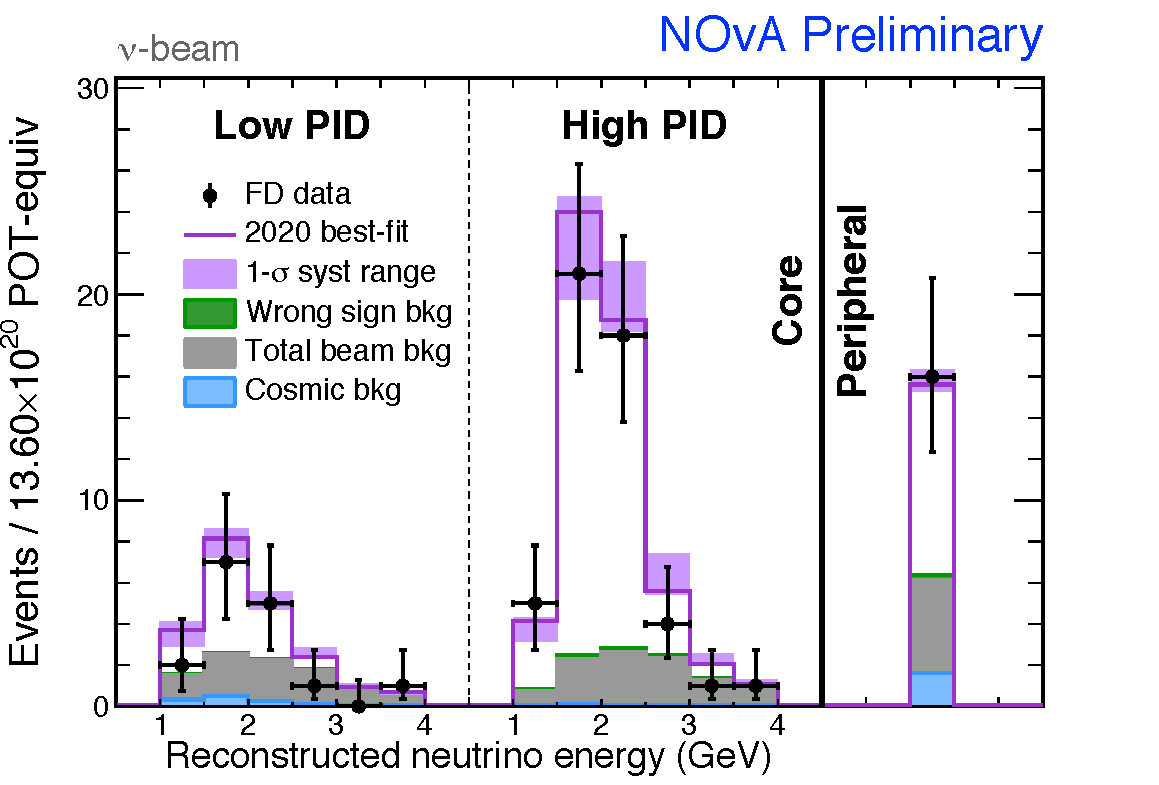
\includegraphics[width=\linewidth]{Chapter_Introduction/Plots/NOvA_NueFD_FHC.pdf}
		\caption{}
		\label{fig:nue20201}
	\end{subfigure}
	\begin{subfigure}{.49\textwidth}
		\centering
		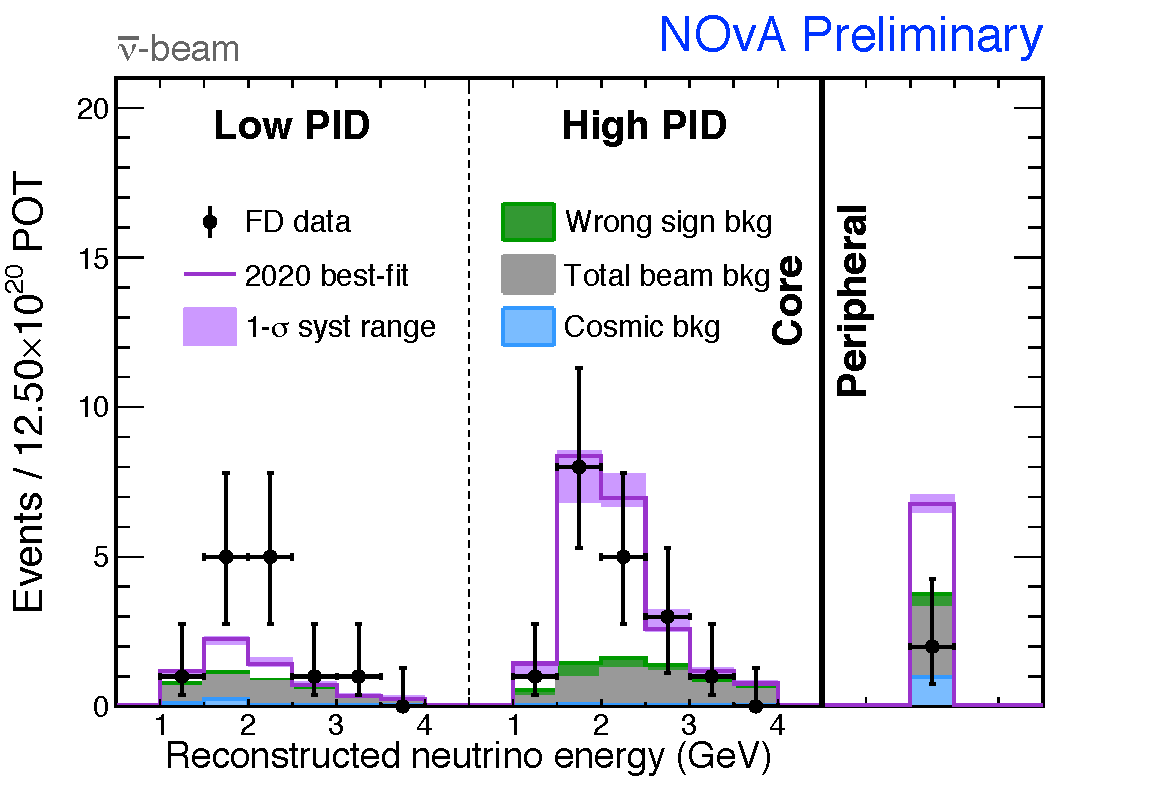
\includegraphics[width=\linewidth]{Chapter_Introduction/Plots/NOvA_NueFD_RHC.pdf}
		\caption{}
		\label{fig:nue20202}
	\end{subfigure} 
	\caption[Here is a short description of the figure.]{Here is a long description of the figure. Taken from~\cite{book:markyT}.}
	\label{fig:nue2020}
\end{figure}

\subsection{Sub-section}
\subsubsection{Sub-sub-section}




%%%%%%%%%%%%%%%%%%%%%%%%%%%%
% ACRONYMS.
\clearpage
\phantomsection
\addcontentsline{toc}{chapter}{Acronyms}
\printglossaries
%%%%%%%%%%%%%%%%%%%%%%%%%%%%


%%%%%%%%%%%%%%%%%%%%%%%%%%%%
% BIBLIOGRAPHY
\clearpage
\phantomsection
\addcontentsline{toc}{chapter}{Bibliography}
\bibliography{Base}
%%%%%%%%%%%%%%%%%%%%%%%%%%%%


%%%%%%%%%%%%%%%%%%%%%%%%%%%%
% START APPENDICES
\appendix
%%%%%%%%%%%%%%%%%%%%%%%%%%%%


%-----------------------------------------------------
% Appendix: A
%-----------------------------------------------------

\chapter{Name of my Appendix}\label{app:a}

\section{Section}




%%%%%%%%%%%%%%%%%%%%%%%%%%%%
% END DOCUMENT
\end{document}
%%%%%%%%%%%%%%%%%%%%%%%%%%%%
